Some astrophysical notation, terms and constants:

\begin{itemize}
    \item $z$ - Redshift, a dimensionless measure of time where $z=0$ denotes the current time and $z \rightarrow \infty$ as we move back in time towards the beginning of the Universe. The redshift also gives the actual physical frequency shift of light emitted from a source moving away from us in an expanding Universe.
    \item $H_{0}$ - The Hubble constant at present time $H(z=0)$, a cosmological constant related to the expansion rate of the Universe. The best measurements of today sets the value of $H_0$ to $67.8\, $ km/s/Mpc \parencite{Planck2016}. Specifically, this means that at $z=0$ a galaxy located 1 Mpc away is receding from us at a velocity of $67.8\,$km/s because of the expansion of the Universe.
    \item $h$ - The ``little Hubble constant'', given by $H_0 = 100\,h\,$km/s/Mpc.
    \item G - The gravitational constant. 
    \item $M_{\ast}$ - The stellar mass of a given galaxy.
    \item $M_{halo}$ - The dark matter halo mass of a given galaxy.
    \item $M_{\odot}$ - Solar mass, the mass of our sun. In astrophysics, masses are always given in units of solar masses.
    \item $L$ - Luminosity. The luminosity of a galaxy is a measure of its total radiated electromagnetic energy per unit time. The absolute magnitude ($\mathcal{M}$) is related to the luminosity as $\mathcal{M} = -2.5 \log(L/L_\odot) + \mathcal{M}_\odot$. With $L_\odot$ and $\mathcal{M}_\odot$ being the solar luminosity and solar magnitude respectively.
    \item $r_{hm}$ - Stellar half-mass radius. The radius within which half the stellar mass of a galaxy is emitted.
    \item $R_e$ - Effective radius. The radius within which half the luminosity of a galaxy is emitted. Is also used to refer to $r_{hm}$ for simulations.
\end{itemize}

\subsection{Galaxy formation}

Our understanding of the formation and evolution of the Universe as a whole is based on the cosmological principle, which states that matter is distributed spatially isotropically and homogeneously across the Universe on large scales. Of course, we would not have any structure formation if the matter was actually perfectly uniformly distributed in the very beginning of the Universe. It is not completely clear how this initial deviation from homogeneity originated, but at very early times after the Big Bang, the Universe was so small that quantum effects would have played a significant role. These tiny quantum fluctuations may then have been responsible for the structure formation we can observe today. Given that these initial density fluctuations in matter were present, gravitational effects will then amplify the overdense regions of space as matter is pulled together. If the Universe did not expand, these instabilities in the density field would just keep growing. However, we know the Universe is expanding, and so the effect is dampened significantly. As matter keeps being pulled in over time, the overdense region might reach a ``turn-around size'' where the gravitational pull is large enough to compensate for the expansion rate of space. Then the matter will collapse towards the center. The exact process for collapse is beyond the scope of this report, but it depends on the ratio of dark matter to baryonic matter, and the properties of the dark matter itself. 

\subsubsection{Dark matter halos}
Dark matter halos are the result of such initial overdense regions of dark matter particles. Halos cover a huge range in magnitude of mass from lower than $10^9 M_{\odot}$ up to sizes of at least $10^{15} M_{\odot}$. In general, halos are ellipsoid in shape. The spherically averaged density profile of halos, as predicted by N-body simulations of dark matter in a $\Lambda$CDM Universe, is well described by the Navarro-Frank-White profile \parencite{Navarro1996}. This profile gives us a halo density ($\rho$) that is proportional to $r^{-1}$ for smaller radii and $r^{-2}$ for large radii,
\begin{equation}
    \frac{\rho}{\rho_{crit}} = \frac{\delta_c}{(r/r_s)(1+r/r_s)^2,}
\end{equation}
where $\rho_{crit} = 3H_0^2/8\pi G$ is the critical density of the Universe, $\delta_c$ is the characteristic overdensity and $r_s$ is the scale radius where the slope changes from $r^{-1}$ to $r^{-2}$. Both $\delta_c$ and $r_s$ may vary for each halo.

Halos grow hierarchically through mergers of smaller halos into larger halos. A smaller halo that merges with a larger halo may survive as a separate entity within the host halo and is then known as a subhalo. 

One of the most interesting properties of a $\Lambda$CDM Universe is the halo mass function, which gives the number density of halos as a function of their mass. In 1974 the halo mass function was defined by William H. Press and Paul Schechter as:

\begin{equation}
    \frac{dn}{dM_{halo}} = f(\sigma)\frac{\overline{\rho}}{M_{halo}^2}\frac{d\log(\sigma^{-1})}{d\log(M_{halo})}.
\end{equation}

Where $\sigma = \sigma (R)$ is the variance of the field with a smoothing radius $R$, $\overline{\rho}$ is the mean density of the Universe and $f(\sigma)$ is the multiplicity function \parencite{Press1974}. 

As an example, Figure \ref{halo_mass} shows the halo mass function found by \textcite{Tinker2008}. In this work, they calculated the halo mass function at $z=0$ based on a set of cosmological simulations (colored points). The solid black lines show the fit to the Schechter function for three different values of $\Delta$, where $\Delta$ is the overdensity within a radius $R_{\Delta}$ with respect to $\rho_{crit}$.

We will not cover the mathematical details of this analytical solution to the mass function, but it is based on the assumption of spherical collapse and depends on both cosmology and redshift.
Until the end of the century, numerical simulations tended to agree with the results presented by Press and Schechter. However, newer and more complex numerical solutions have shown that the Press-Schechter formalism tends to overestimate the amount of smaller halos, while under-predicting the abundance of larger halos.

\begin{figure}
    \centering
    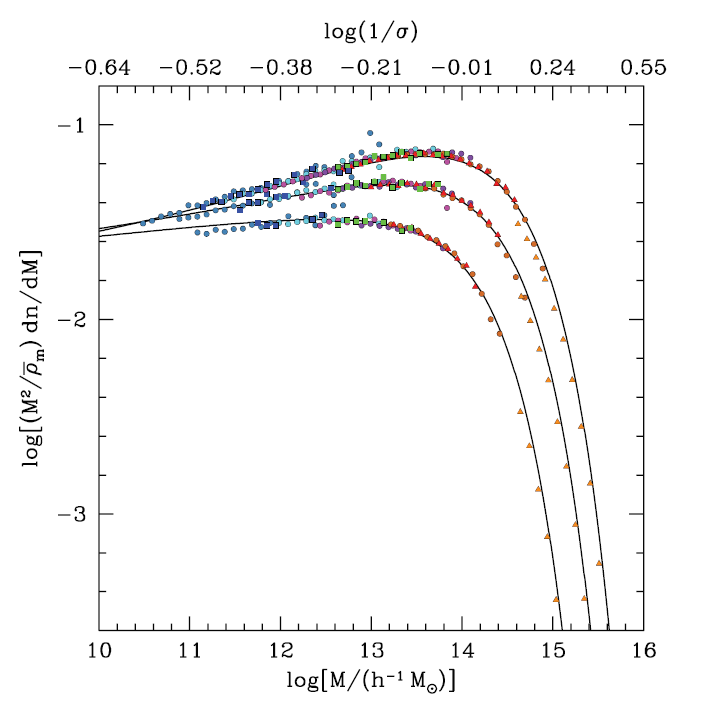
\includegraphics[width=0.9\textwidth]{images/halo_mass_function.png}
    \caption{Halo mass function for three different overdensities, $\Delta = 200, 800, 3200$ from top to bottom (points). The different points represent the different simulations used. The solid black lines are best fits for each value of the overdensity $\Delta$. They are all three Schechter functions, with varying multiplicity functions to get the best fit to their respective data points. Credit \textcite{Tinker2008}.}
    \label{halo_mass}
\end{figure}

\subsubsection{Galaxies}
Dark matter halos formed before baryonic matter could gather in densities even close to that needed to form stars, as there is 6-7 times more dark matter than baryonic matter. The dark matter halos created a gravitational potential well which gave room for the primordial baryonic matter (ionized hydrogen gas) to start collapsing. 

As the density of the gas increases, temperature increases and halts the collapse, but through several radiation cooling processes the gas is able to collapse enough for fusion to start and stars to be born. Because of the halos role as initial potential wells, the baryonic matter collapses in such a way that the angular momentum of its initial components get transferred to the galaxy as a whole, and the result is a rotating disk galaxy at the center of the halo. This is the birth process of galaxies.

Galaxies are mainly composed of stars and hot gas, with a smaller contribution of stellar remnants, cold gas and dust. Hot gas is hydrogen gas that is fully ionized and does not collapse into stars, while cold gas has a much lower temperature and can contribute to star formation. There are at least two trillion galaxies in the observable Universe \parencite{Conselice2016}, with stellar masses ranging from less than $10^6 M_{\odot}$ to $10^{12} M_{\odot}$ and larger. 

It has been found that a large fraction of galaxies are gravitationally bound to each other in groups and clusters.
Galaxy clusters are the largest gravitationally bound systems in the Universe, and can span a distance of several megaparsecs. They typically contain more than a hundred galaxies, as well as large amounts of intergalactic gas. Galaxies in clusters serve an important purpose to astrophysicists, as they essentially function as tracers of the largest halos in the Universe.

As galaxies reside in the center of halos, they too follow a hierarchical growth pattern where larger galaxies are created through the merger of smaller galaxies. All galaxies start of as disk galaxies, so galaxies that have an elliptical component of stars and gas with pressure dominated random motions and which extends in all directions from the center, are results of the merging of galaxies. In galaxy clusters the density of galaxies is much higher than the average of the Universe, so the likelihood of a galaxy merger is higher there. Therefore clusters contain a higher percentage of elliptical galaxies.

A very important property of the galaxy population is the galaxy luminosity function, which gives the number density of galaxies as a function of their luminosity. The luminosity of a galaxy is directly proportional to its stellar mass, so the luminosity function also gives us the mass distribution of galaxies. Mathematically, the luminosity function is defined as $\phi(L)dL$, where $\phi(L)dL$ is the number density of galaxies in the luminosity range $L \pm dL/2$. In 1976 Paul Schechter proposed a fit to the luminosity function of galaxies on the form

\begin{equation} \label{lum_func}
    \phi(L)dL = \phi^*(L/L^*)^{\alpha}\exp{(-L/L^*)}dL/L^*,
\end{equation}

where $\phi^*$ is a normalization, $L^*$ is the characteristic luminosity for that sample of galaxies (it will differ for instance for galaxies within a cluster compared to isolated galaxies) and $\alpha$ is the slope of the power law where $L<<L^*$ \parencite{Schechter1976}. Figure \ref{luminosity_function} shows the luminosity function (points) as well as the best fit for equation \ref{lum_func} (solid line). This Schechter function is still a good fit to this day, and is in excellent agreement for galaxies with $L>>L^*$. For the low mass range of galaxies, the parameter $\alpha$ must be found, and this is one of the challenges of astrophysicists that study galaxy properties.

\begin{figure}
    \centering
    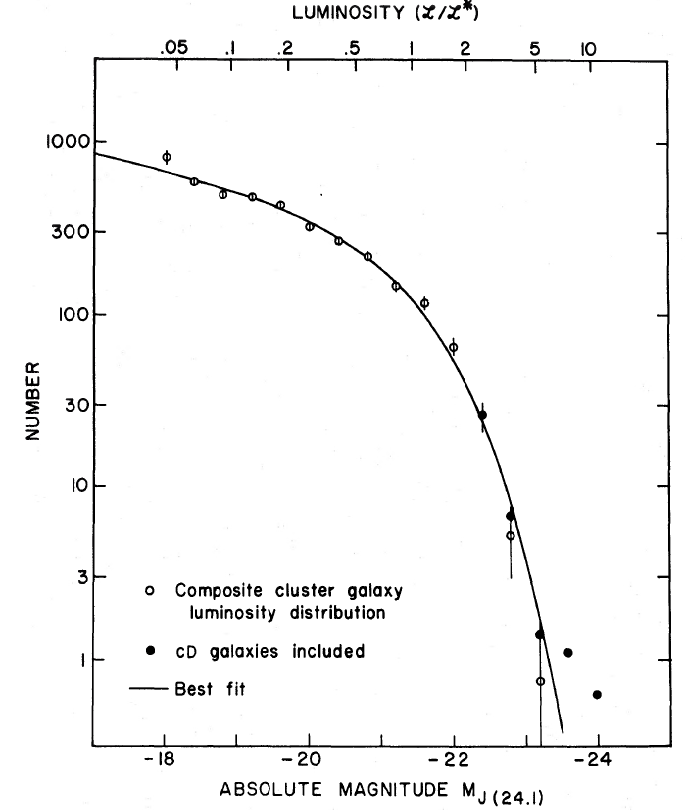
\includegraphics[width=0.9\textwidth]{images/luminosity_function.png}
    \caption{The luminosity function at redshift 0. The open circles correspond to observed galaxies in clusters, while the filled in circles denote cD galaxies (giant ellipticals). The solid line shows the best fit using equation \ref{lum_func}. Credit: \textcite{Schechter1976}.}
    \label{luminosity_function}
\end{figure}

\subsubsection{The Stellar-to-Halo mass relation}

The Stellar-to-Halo mass relation (hereafter, SHM relation) gives the stellar mass of a galaxy as a function of its host halo mass. This is particularly difficult to determine empirically, as it is not possible to directly measure the dark matter halo mass.

One way of looking for this relation is through a method called abundance matching. In abundance matching, the numerically found halo mass function and the observationally found luminosity function are combined. This is done using the simple assumption that the largest halo contains the largest galaxy, the second largest halo contains the second largest halo and so on. By mapping each galaxy to its corresponding halo in such a fashion, the shape of the SHM relation can be found directly.

Using abundance matching, the SHM relation has been found to be well described by a double power law with different slopes for the low-mass and high-mass end of the spectrum \parencite{Behroozi2013}. 

Other ways of studying the SHM relation could be through simulations which include halo and stellar mass like IllustrisTNG, or inferring the halo mass empirically by using the rotational curves of disk galaxies (see Section \ref{lates}), gravitational lensing and other mobservational methods.

\subsection{Galaxy evolution and classification}

As soon as telescopes became good enough to clearly make out galaxies in the sky, it became apparent to astronomers that galaxies come in many different shapes and sizes. The morphology of the galaxy is closely linked to other properties of the galaxy and is therefore important for the classification of galaxies. Edwin Hubble classified galaxies on a spectra \parencite{Hubble1926}, with elliptical galaxies (galaxies that have a dominant spheroidal component) on one end of the spectrum and spiral galaxies (galaxies with a prominent disk component) on the other (Figure \ref{hubble}). The galaxy types were presented as a sequence, so Hubble deemed it convenient to use the adjectives ``early'' and ``late'' to describe the two extreme ends of the spectrum. He did consider the fact that these words might be confusing because of their temporal connotations, but went ahead with using ``early'' and ``late'' as a proxy for ``less complex'' and ``more complex'', respectively. Indeed this turned out to be confusing, as it is now established that galaxies actually evolve with time along the sequence, starting out as late type disk galaxies and often ending up as more massive early type ellipticals.

\begin{figure}
    \centering
    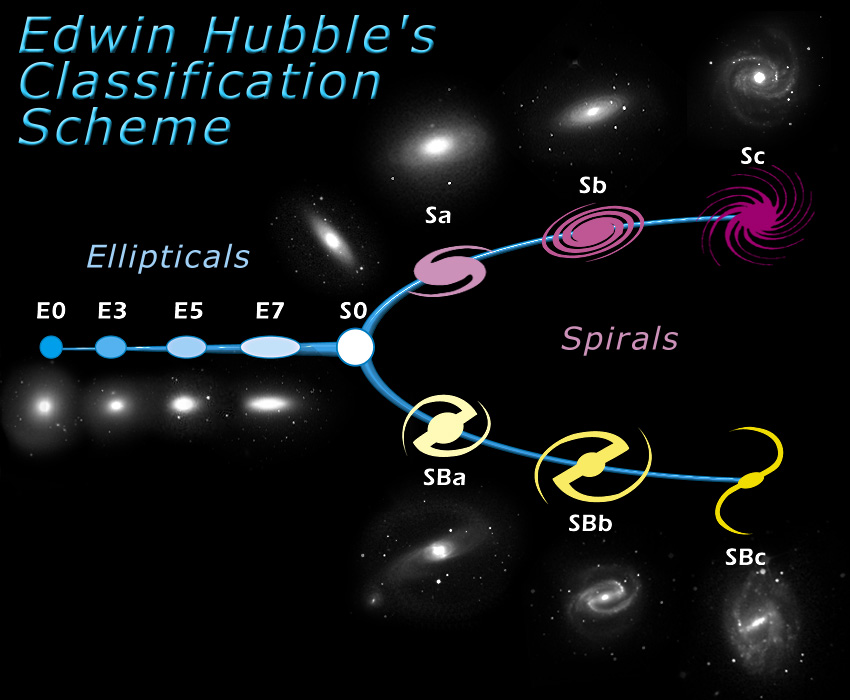
\includegraphics[width=0.7\textwidth]{images/hubble.jpg}
    \caption{Chart from 1999 showing the original classifications of galaxy morphology. Credit: ESA/Hubble}
    \label{hubble}
\end{figure}

In the $\Lambda$CDM model, galaxies grow through mergers. Mergers are separated into two types, major and minor mergers. Major mergers are events where two galaxies of equal size collide and become one galaxy, while minor mergers happen when one of the galaxies is significantly smaller than the other. Simulations have shown that a major merger between two disk galaxies produces an elliptical. The Milky Way, which is a large ($M_*>10^{10} M_\odot$) spiral galaxy has probably grown through many smaller minor mergers, and thus kept its disky shape.

It is not always easy to distinguish between a disky elliptical and a spiral with a large spheroidal component (bulge). Some galaxies are also in the middle of a merging process. These can have very irregular shapes, and so are hard to classify. Other galaxies are very small, so called dwarf galaxies. These galaxies tend to have very little stellar mass compared to dark matter, so they do not exhibit the properties of ellipticals, even though they may be more elliptical in shape.

Galaxies were initially seperated into the two types (early and late) by their shape, but as astronomers have studied these different galaxy categories, it has become apparent that there are many other properties that also serve to distinguish the two types. Table \ref{morphologies} gives a quick overview of the main properties of early and late type galaxies, while the rest of this Section explains them in more detail.


\begin{table}
\begin{center}
\caption{Galaxy properties by morphology type.}
\label{morphologies}
\begin{tabular} { l| c c } 
 \hline
 \hline
  & Early type & Late type \\
 \hline
 Shape & Spheroidal & Disk \\
 Color & Red & Blue \\
 Velocity direction& Radial & Circular \\
 Stellar population & Older & Younger \\
 Star formation rate & Low & High \\
 Size & Smaller & Larger \\
 Gas and dust & Little & More \\
  
 \hline 
\end{tabular}
\end{center}
\end{table}

\subsubsection{Elliptical (early type) galaxies}
Elliptical galaxies are mainly pressure-dominated systems, meaning that the motion of the stars is predominantly radial. The largest galaxies in the Universe tend to be ellipticals, but they come in all sizes. The star population of ellipticals is generally older than that of spirals, and there is usually little to no star formation. There is very little gas and dust in ellipticals, and they tend to emit more light in the redder end of the electromagnetic spectrum. Early type galaxies are less common than late type galaxies, and are more usually found in galaxy clusters.

\subsubsection{Spiral (late type) galaxies} \label{lates}
Late type galaxies have a prominent disky component which orbits around the galaxy's center. The rotational velocity of the disk is typically larger than the velocity dispersion of the galaxy's bulge. The stars in a spiral galaxy are usually younger than those in early types. There is a lot of gas and dust present in spirals, giving rise to ongoing star formation. Late type galaxies are bluer in color than early types. Field galaxies, which are not part of any galaxy cluster, are predominantly spirals. 


The rotational velocities of the stars at different radii in the disk of spiral galaxies can be measured observationally, and plotting the velocity as a function of radius gives us the velocity curve of the galaxy. If the mass in the galaxy was solely made up of the gas and stars that we are able to detect optically, we would expect the velocity curve to drop off as we get to the outer parts of the galaxy. Assuming the particles move in circular orbits around the center of mass, the circular velocity at a given radius is given by the formula

\begin{equation}
    v_{circ} = \sqrt{GM(<R)/R}, 
\end{equation}

where $M(<R)$ is the total mass within radius $R$. However, the observational data shows that the velocity curve does not fall off towards the outer parts of the galaxy, but actually flattens out. An example of this can be seen in Figure \ref{rotation_curves}. There the rotation curves of several spiral galaxies are shown, along with the curve showing the expected fall off of velocity if there was no dark matter (long-dashed line). This perplexed early astrophysicists, as the mass inside the outer radius must be much greater than that which could be accounted for by the stars and gas in the galaxy. An effort to solve this problem led to the theory of dark matter, and later to the $\Lambda$CDM model.

\begin{figure}
    \centering
    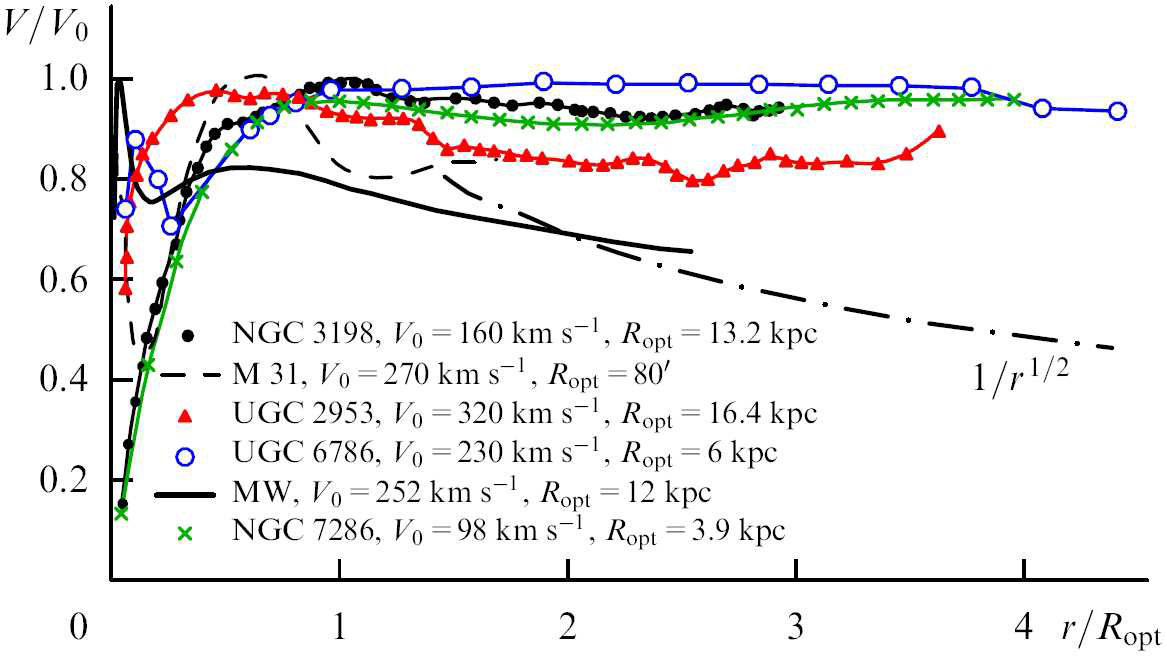
\includegraphics[width=0.9\textwidth]{images/rotation_curves.png}
    \caption{Rotation curves for several spiral galaxies (points). The velocities are normalized with respect to each of the galaxies maximum velocity. Radial distances are in units of the optical radius $R_{opt}$ (the radius within 83\% of the light is enclosed). The long-dashed line shows the expected Keplerian curve if there was no dark matter. Credit: \textcite{Zasov2017}.}
    \label{rotation_curves}
\end{figure}

\subsubsection{Classifying galaxies}

An important factor in many studies of galaxy formation and evolution is looking at and comparing the properties of the two main morphological types of galaxies. In observations, a visual classification method is usually used, although it is intensively time-consuming. %you can cite here galaxy zoo (https://www.zooniverse.org/projects/zookeeper/galaxy-zoo/) 
Other methods have therefore been devised for identifying early and late-type galaxies in simulations. In many studies, several classification methods are used in conjunction. 

As early-type galaxies have much less cold gas than late-type galaxies, a simple division in the galaxy population based on the gas fraction (gas mass divided by stellar mass) will be effective at roughly separating the two types. Gas is not distributed evenly in galaxies however, so it is important to consider the physical volume where the gas fraction is calculated. A large volume will inevitably contain more hot (not star-forming) gas and potentially allow for early-type galaxies to be considered as late types. Late-type galaxies also have a wide range of gas fractions. The most massive spiral galaxies ($M_\ast \sim 10^{11} M_\odot$) can contain as little as 5\% gas, while low-mass disks ($M_\ast < 10^{9.5} M_\odot$) can contain up to 80\% \parencite{Mo2010}. In \textcite{Ferrero2020} gas fraction was used as one of two criteria of morphological classification. Galaxies with a gas fraction of less than 0.1 were considered for early types, while those with more were potential candidates for late-type classifications.

Another way of separating galaxies into the early and late-type categories is by using the specific star formation rate (sSFR). The sSFR of a galaxy is the galaxy's star formation rate divided by the stellar mass content of the galaxy. As an example, a galaxy with a stellar mass of $10^{10} M_\odot$ that produces stars with a total mass $1 M_\odot$ has a sSFR of $10^{-10}$, commonly expressed as $\log(sSFR) = -10$. Galaxies are tagged as ``quenched'' or ``main-sequence'', where quenched galaxies have little to no star formation, while main-sequence galaxies have a significant amount of star formation \parencite{Noeske2007}. More formally, they are separated by how far from the ridge of the star-formation main-sequence they are found. In a study using the data from the TNG simulation, \textcite{Genel2017} defined the ridge of the main-sequence as the mean of the sSFR for galaxies with mass $10^{9} M_{\odot} < M_* < 10^{10.5} M_{\odot}$, and takes a value of $\log (sSFR[Gyr^{-1}]) = -0.94$ for $z=0$. Galaxies are then considered `main-sequence' if their sSFR are within 0.5 dex of this value. A simpler criteria for main-sequence galaxies is to drop the upper bound and include all galaxies that have sSFR more than 0.5 below the ridge. ``Quenched'' galaxies are defined as those with sSFR at least 1 dex below the ridge. 

A common way of estimating a galaxy's ``diskyness'' is to use the rotational ($K_{rot}$) to total ($K$) kinetic energy parameter $\kappa_{rot}$. 
\begin{equation}
    \kappa_{rot} = \frac{K_{rot}}{K} = \frac{\sum_{i=1}^{N} m_i (j_{z, i}/R_i)^2}{\sum_{i=1}^{N} m_i v_i^2},
\end{equation}
where $j_{z, i}$ is the z-component of the specific angular momentum ($\vec{j} = \vec{r} \times \vec{v}$), $m_i$ is the mass, and $R_i$ is the projected radius of stellar particle $i$ in the xy-plane. 
This value indicates how much of the kinetic energy of the galaxy is invested in the ordered rotation about its axis. To calculate $\kappa_{rot}$, the axis of rotation must first be found. The galaxy is then rotated such that the z-axis of the galaxy's coordinate system is pointed in the direction of the axis of rotation, and $\kappa_{rot}$ is calculated.
For a perfect disk galaxy that is totally rotationally supported $\kappa_{rot} = 1$, while for a totally pressure supported system, $\kappa_{rot}$ would approach zero. In \textcite{Sales2012}, galaxies were classified as early type if they had $\kappa_{rot} < 0.5$ and late type for $\kappa_{rot} > 0.7$. This leads to a significant amount of ``intermediate types'', but other works have simply made use of a single cut at $\kappa_{rot} = 0.6$ \parencite{Ferrero2020}. Figure \ref{kappa_rot} shows the face-on and edge on structure of three rotated galaxies with varying values of $\kappa_{rot}$. The higher the rotational to kinetic energy ratio, the more disk shaped is the galaxy.


\begin{figure}
    \centering
    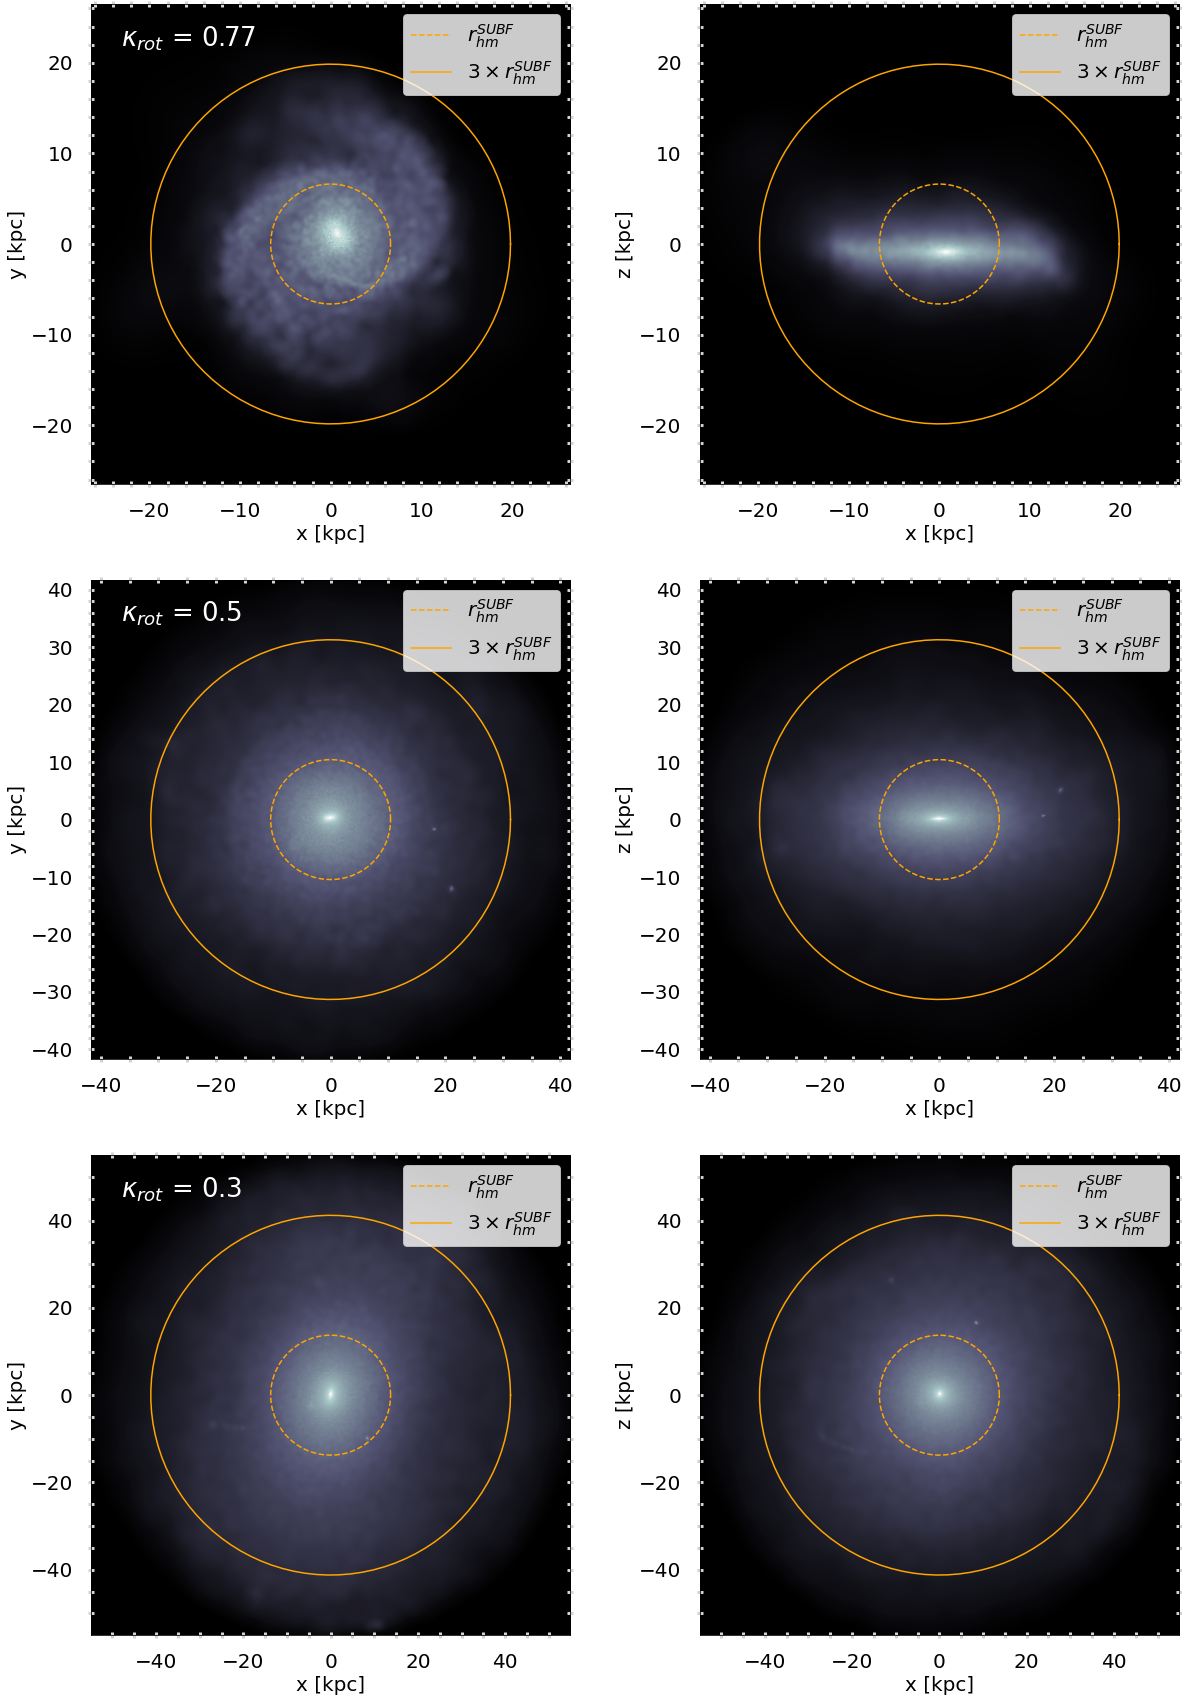
\includegraphics[width=0.85\textwidth]{images/kappa_rot.png}
    \caption{The stellar mass density projections of three different galaxies with $\kappa_{rot} =$ 0.77, 0.5 and 0.3, from top to bottom. The galaxies are shown both face on (right) and edge on (left).}
    \label{kappa_rot}
\end{figure}

\subsection{Galaxy properties}
In this report I will be looking at many of the main galaxy properties that have been explored throughout the years. We will only be looking at the relations in the present time, $z=0$, but the relations have been studied across redshifts and many are redshift-dependent.

\subsubsection{The Tully-Fisher relation}

\textcite{TullyFisher1977} found a surprisingly good correlation between the luminosity of a spiral galaxy and the characteristic rotational speed of its disk on the form of a simple power law with index $\alpha$,

\begin{equation}
    L \propto V_{rot}^\alpha.
\end{equation}

This is known as the Tully-Fisher relation (TFR) (Figure \ref{tully_fisher}). As stellar mass is directly proportional to the luminosity, this gives us the ability to estimate stellar mass from a simple measurement of the rotational velocity.

\begin{equation}
    M_* \propto V_{rot}^\alpha 
\end{equation}

$\alpha$ was found to be 3.7 \parencite{TullyFisher1977}. Later work has found $\alpha$ to lie between 3 and 4 \parencite{Lelli2019, Bloom2017}.

This relation is a great tool for estimating the distance to a galaxy, as the predicted total luminosity can be compared to the apparent magnitude at Earth. For numerical simulations, being able to reproduce the TFR is an essential way to check if the model is reliable.

\begin{figure}
    \centering
    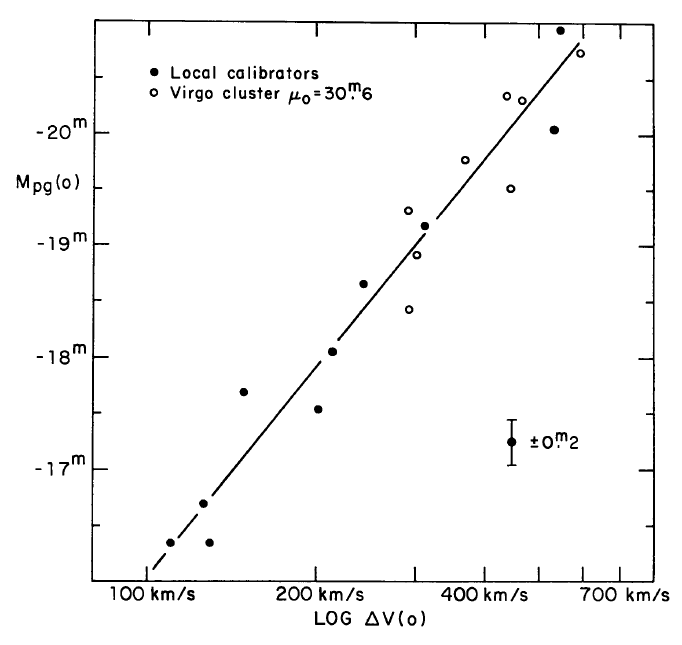
\includegraphics[width=0.9\textwidth]{images/tully_fisher.png}
    \caption{The original figure from the 1977 paper by R.B. Tully and J.R. Fisher, showing the linear fit for the luminosity - velocity values in the log-log plane. Credit: \textcite{TullyFisher1977}}
    \label{tully_fisher}
\end{figure}

\subsubsection{The Faber-Jackson relation and the Fundamental Plane}
At around the same time \textcite{TullyFisher1977} linked the velocity dispersion and luminosity of early type galaxies. In observations, the only velocities of the components of a galaxy we can measure are the line-of-sight velocities ($V$). These are calculated using the observed Doppler shift in the galactic spectrum. The velocity dispersion of a galaxy is then defined as the standard deviation of the line-of sight velocities.

\begin{equation} \label{standard_dev}
    \sigma^{2} = \frac{1}{N} \sum_{n=1}^{N} (V_{i} - \overline{V})^2
\end{equation}

The proposed relation between $\sigma$ and $L$ was on the form of a power law as well,

\begin{equation}
    L \propto \sigma^{\gamma},
\end{equation}

with a power law index $\gamma$ of approximately 4 (Figure \ref{faber_jackson}).

\begin{figure}
    \centering
    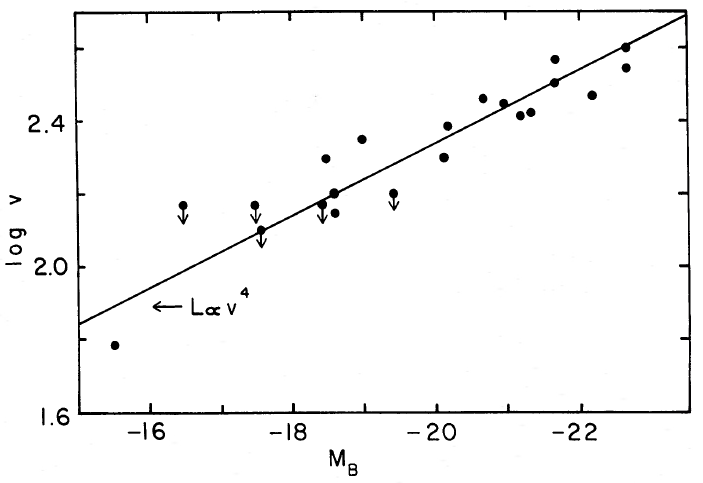
\includegraphics[width=0.9\textwidth]{images/faber_jackson.png}
    \caption{The original fit for the Faber-Jackson relation as presented in the 1976 paper. It shows the velocity dispersion as function of the luminosity in the log-log plane (dots), along with a power law with index 4 (solid black line). Credit: \parencite{TullyFisher1977}}
    \label{faber_jackson}
\end{figure}

This is known as the Faber-Jackson (FJ) relation. The scatter in the FJ relation was larger than that found for the TFR however, and it was later found that the velocity dispersion was dependent on the size of the galaxy. This dependency also took the form of a power law, and so the velocity dispersion is more accurately described by the function

\begin{equation}
    \sigma \propto L^a R^b.
\end{equation}

With the radius added into the equation, the scatter became much less significant. Most ellipticals are found on the same plane in ${\sigma, R, L}$ space. This became known as the Fundamental Plane (FP) \parencite{Djorgovski1987}, and is also something which successful numerical simulations must reproduce.

\subsubsection{Color bimodality}
Color, in astrophysics, is defined as the difference in magnitudes measured for a galaxy by two different optical filters. A galaxy that is "blue" has a larger amount of blue light than red. In general, galaxies are found to inhabit one of two groups on a color-mass diagram, blue or red (see Figure \ref{color_bimodality}). The blue galaxies are most often late type galaxies, while the red ones are mainly early types. There are many factors that contribute to the color of a galaxy, like stellar age and metallicity as well as the amount of gas the light has passed through and its metallicity.

\begin{figure}
    \centering
    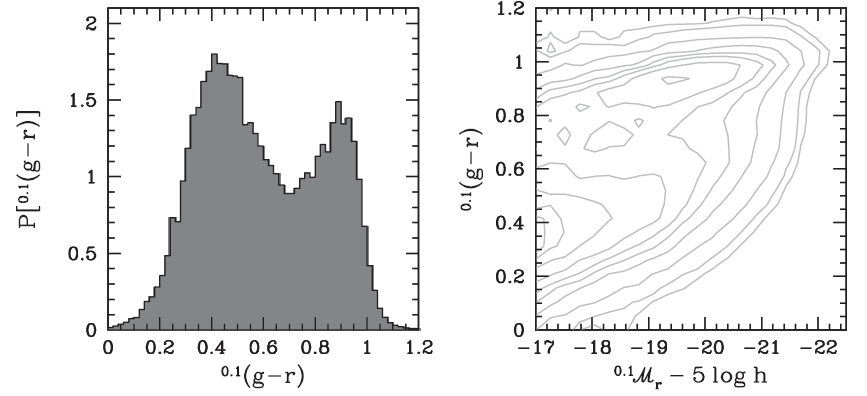
\includegraphics[width=0.9\textwidth]{images/color_bimodality.png}
    \caption{To the left: The probability density of the g-i color for over 350 000 galaxies in the Sloan Digital Sky Survey. To the right: The color-magnitude contour map for the same galaxies, clearly showing two distinct populations. Credit: \textcite{Mo2010}}.
    \label{color_bimodality}
\end{figure}

